\subsection{Breitgefächerte Anwendungen}
\subsubsection*{Aus der Geometrie}
\begin{bsp}
    {Kippende Schale - Aufgabe 155 im Buch}{}
    Eine auf dem Gartentisch liegende Halbkugelschale aus Glas ist randvoll mit Wasser gefüllt. Um welchen Winkel muss die Schale geneigt werden, damit exakt die Hälfte des Wassers ausfliesst?
    \begin{center}
        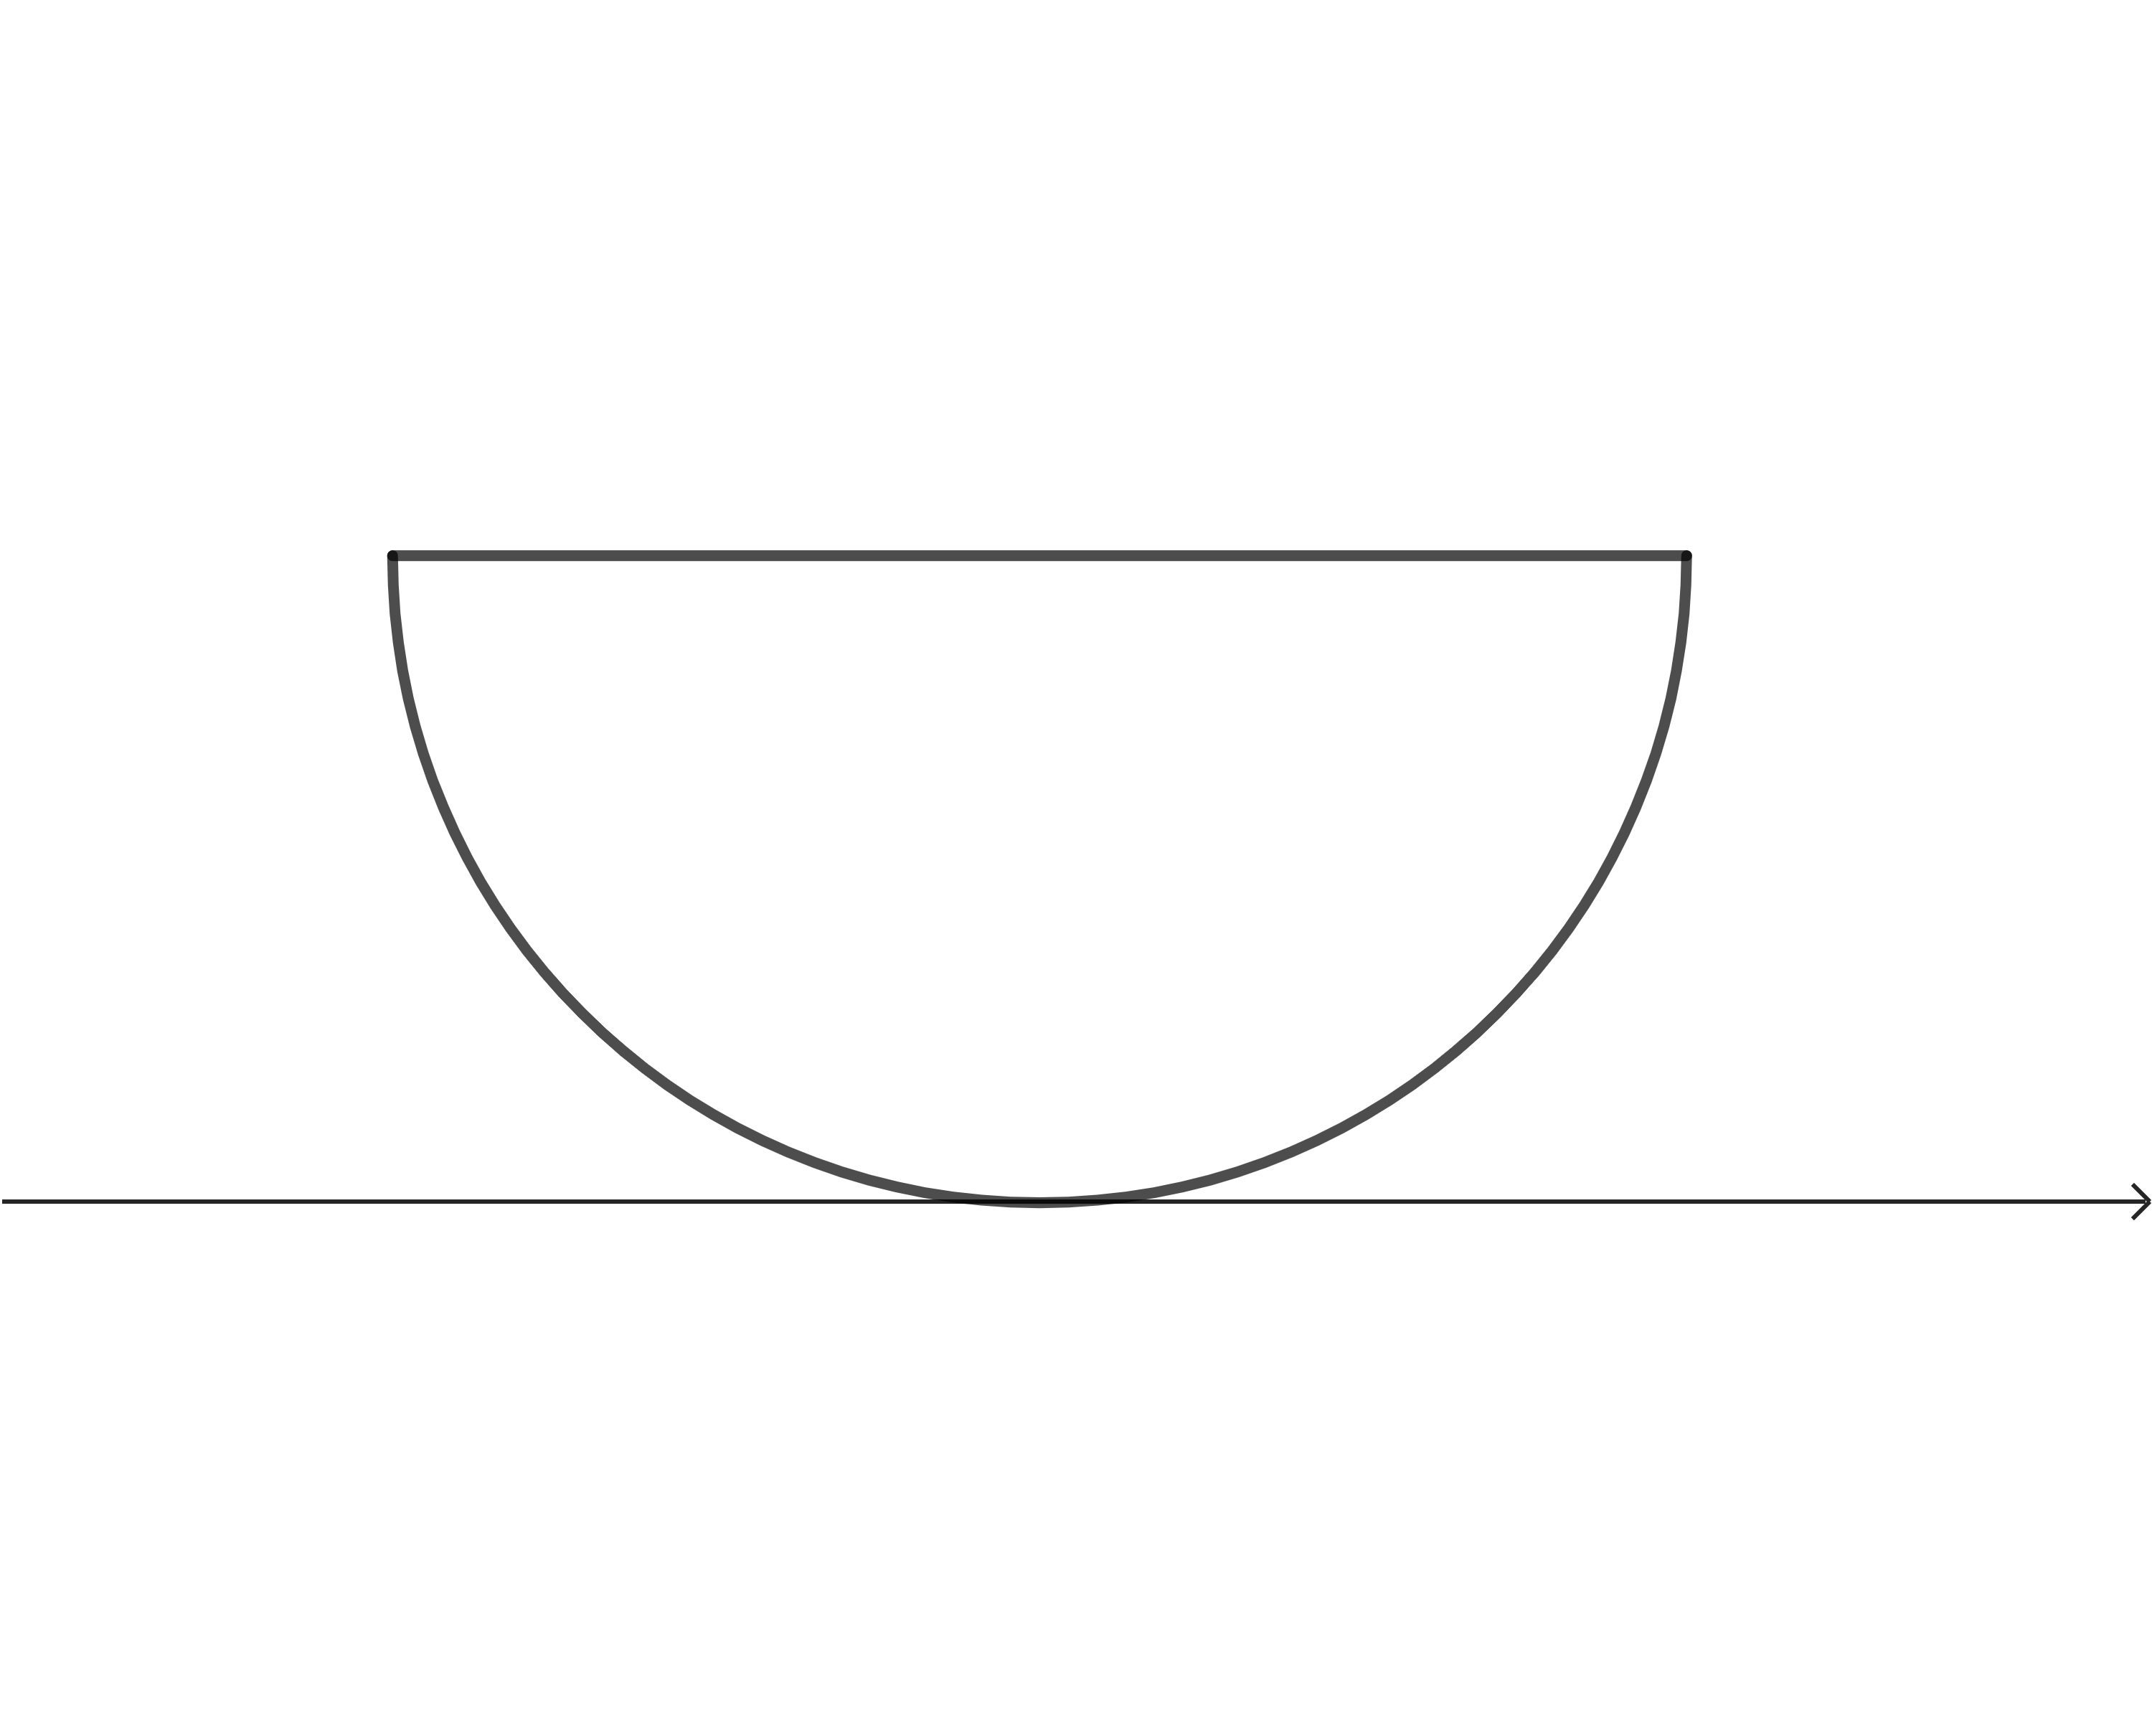
\includegraphics[width = 0.4\textwidth]{media/DMK155-1.png}\hfill
        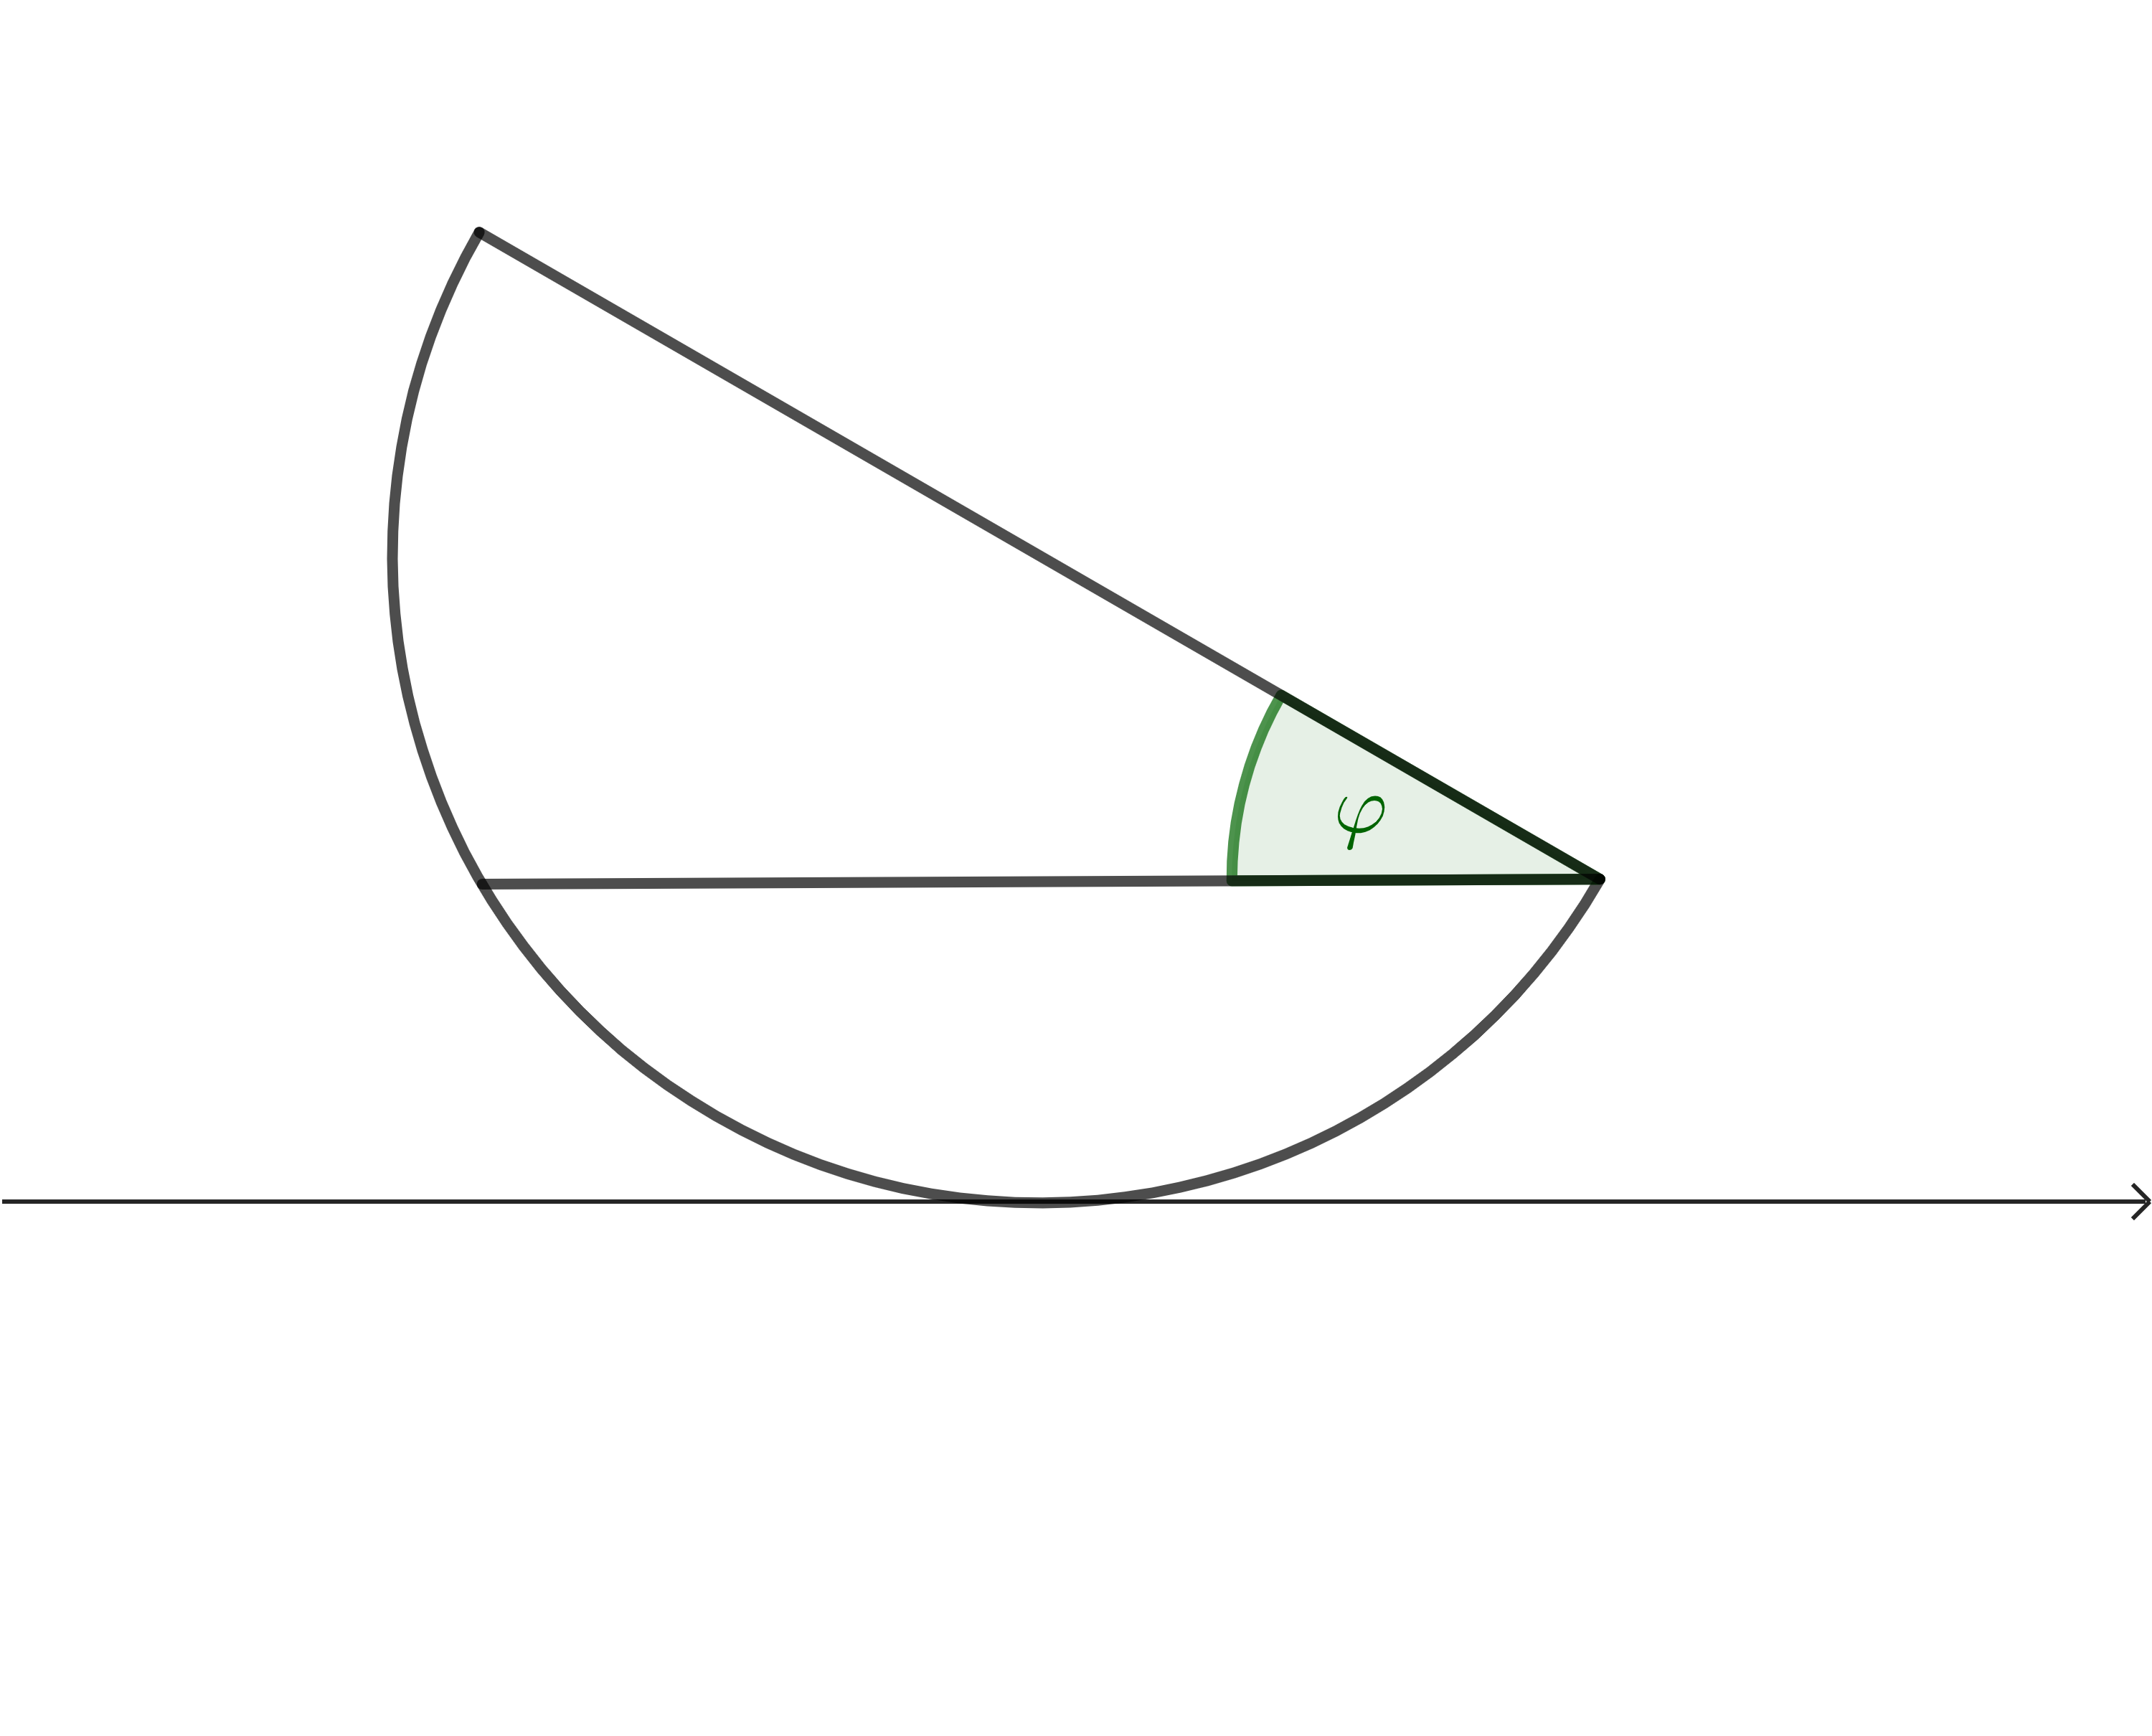
\includegraphics[width = 0.4\textwidth]{media/DMK155-2.png}
    \end{center}
\end{bsp}
\clearpage
\subsubsection*{Aus der Physik}

Wenn ein Körper sich mit konstanter Geschwindigkeit bewegt, lässt sich der zurückgelegte Weg als das Produkt aus Zeit und Geschwindigkeit berechnen:
$$ \Delta  s = v\cdot \Delta t$$
Grafisch kann das Produkt aus Zeit und Geschwindigkeit als Flächeninhalt interpretiert werden:
\begin{center}
    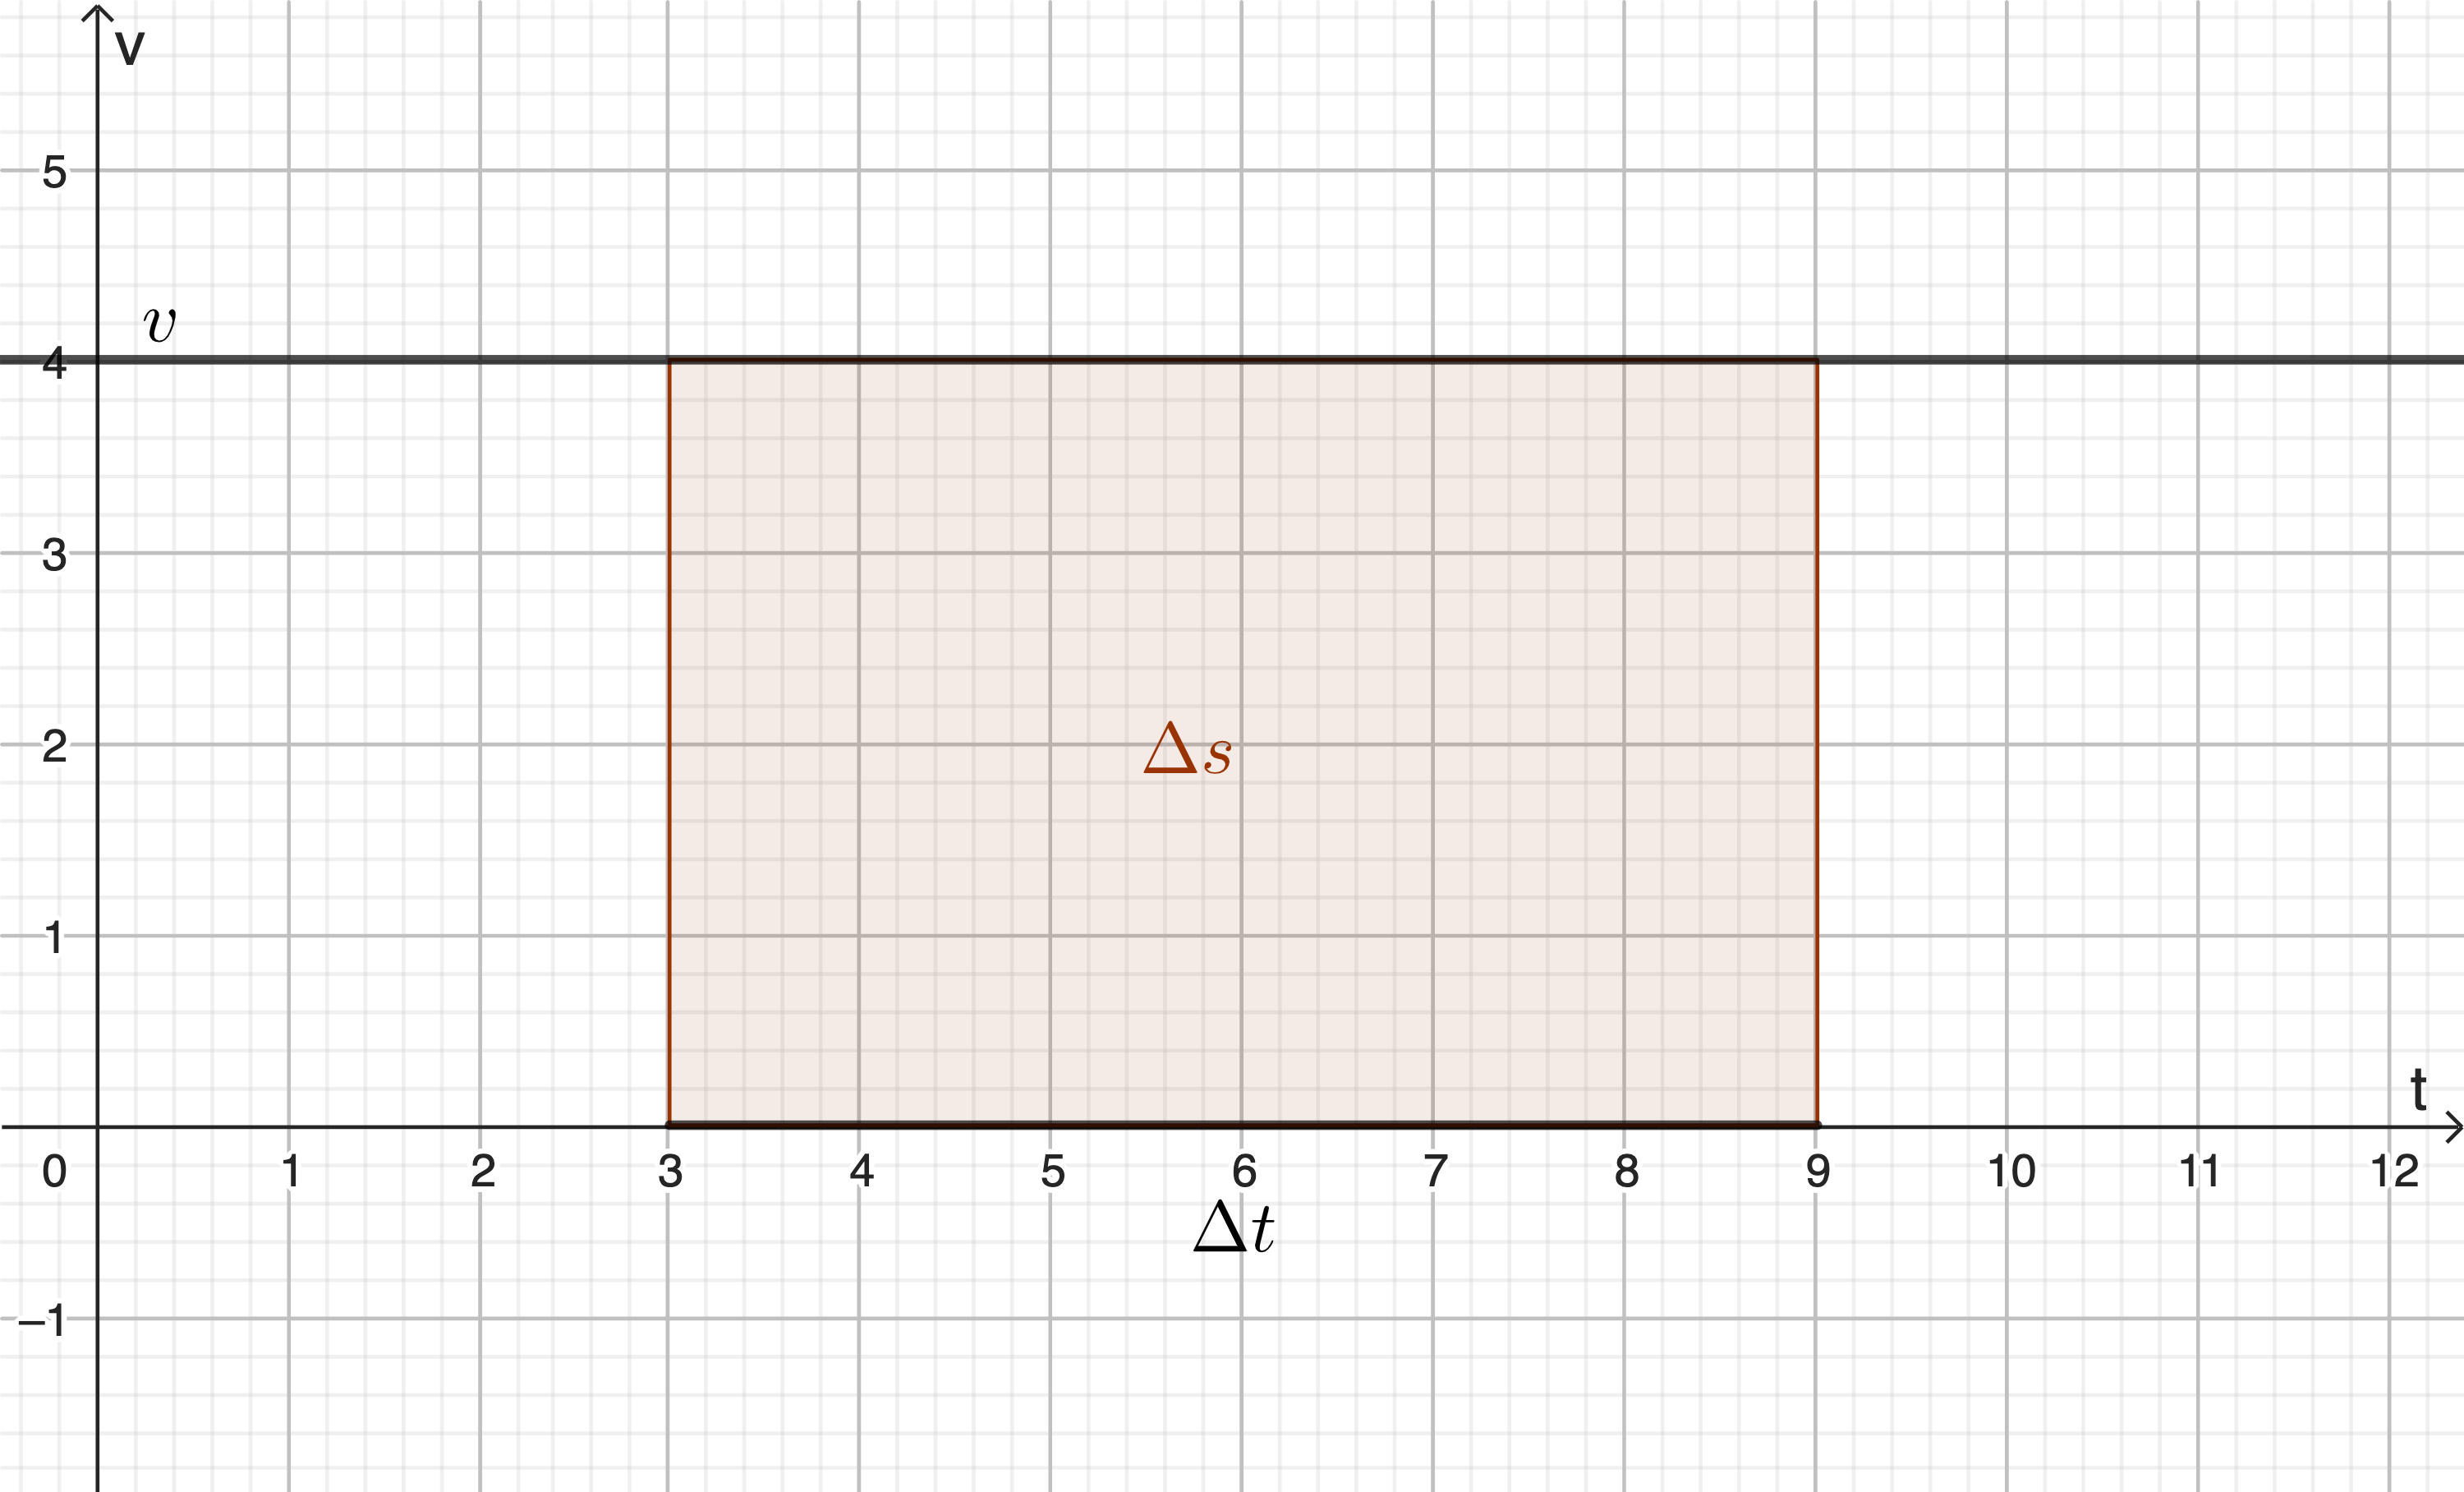
\includegraphics[width = 0.5\textwidth]{media/WegAlsIntegral1.png}
\end{center}

Etwas schwieriger wird es, wenn die Geschwindigkeit nicht konstant ist. Betrachten wir ein Körper, dessen Geschwindigkeit linear wächst: $v(t) = a\cdot t$. Welchen Weg legt der Körper im Zeitintervall $[t_1, t_2]$ zurück?

Um den zurückgelegten Weg näherungsweise zu berechnen, teilen wir das Zeitintervall $[t_1, t_2]$ in viele kleine Intervalle und nehmen an, dass in diesen kleinen Zeitintervallen die Geschwindigkeit näherungsweise konstant ist:
\begin{center}
    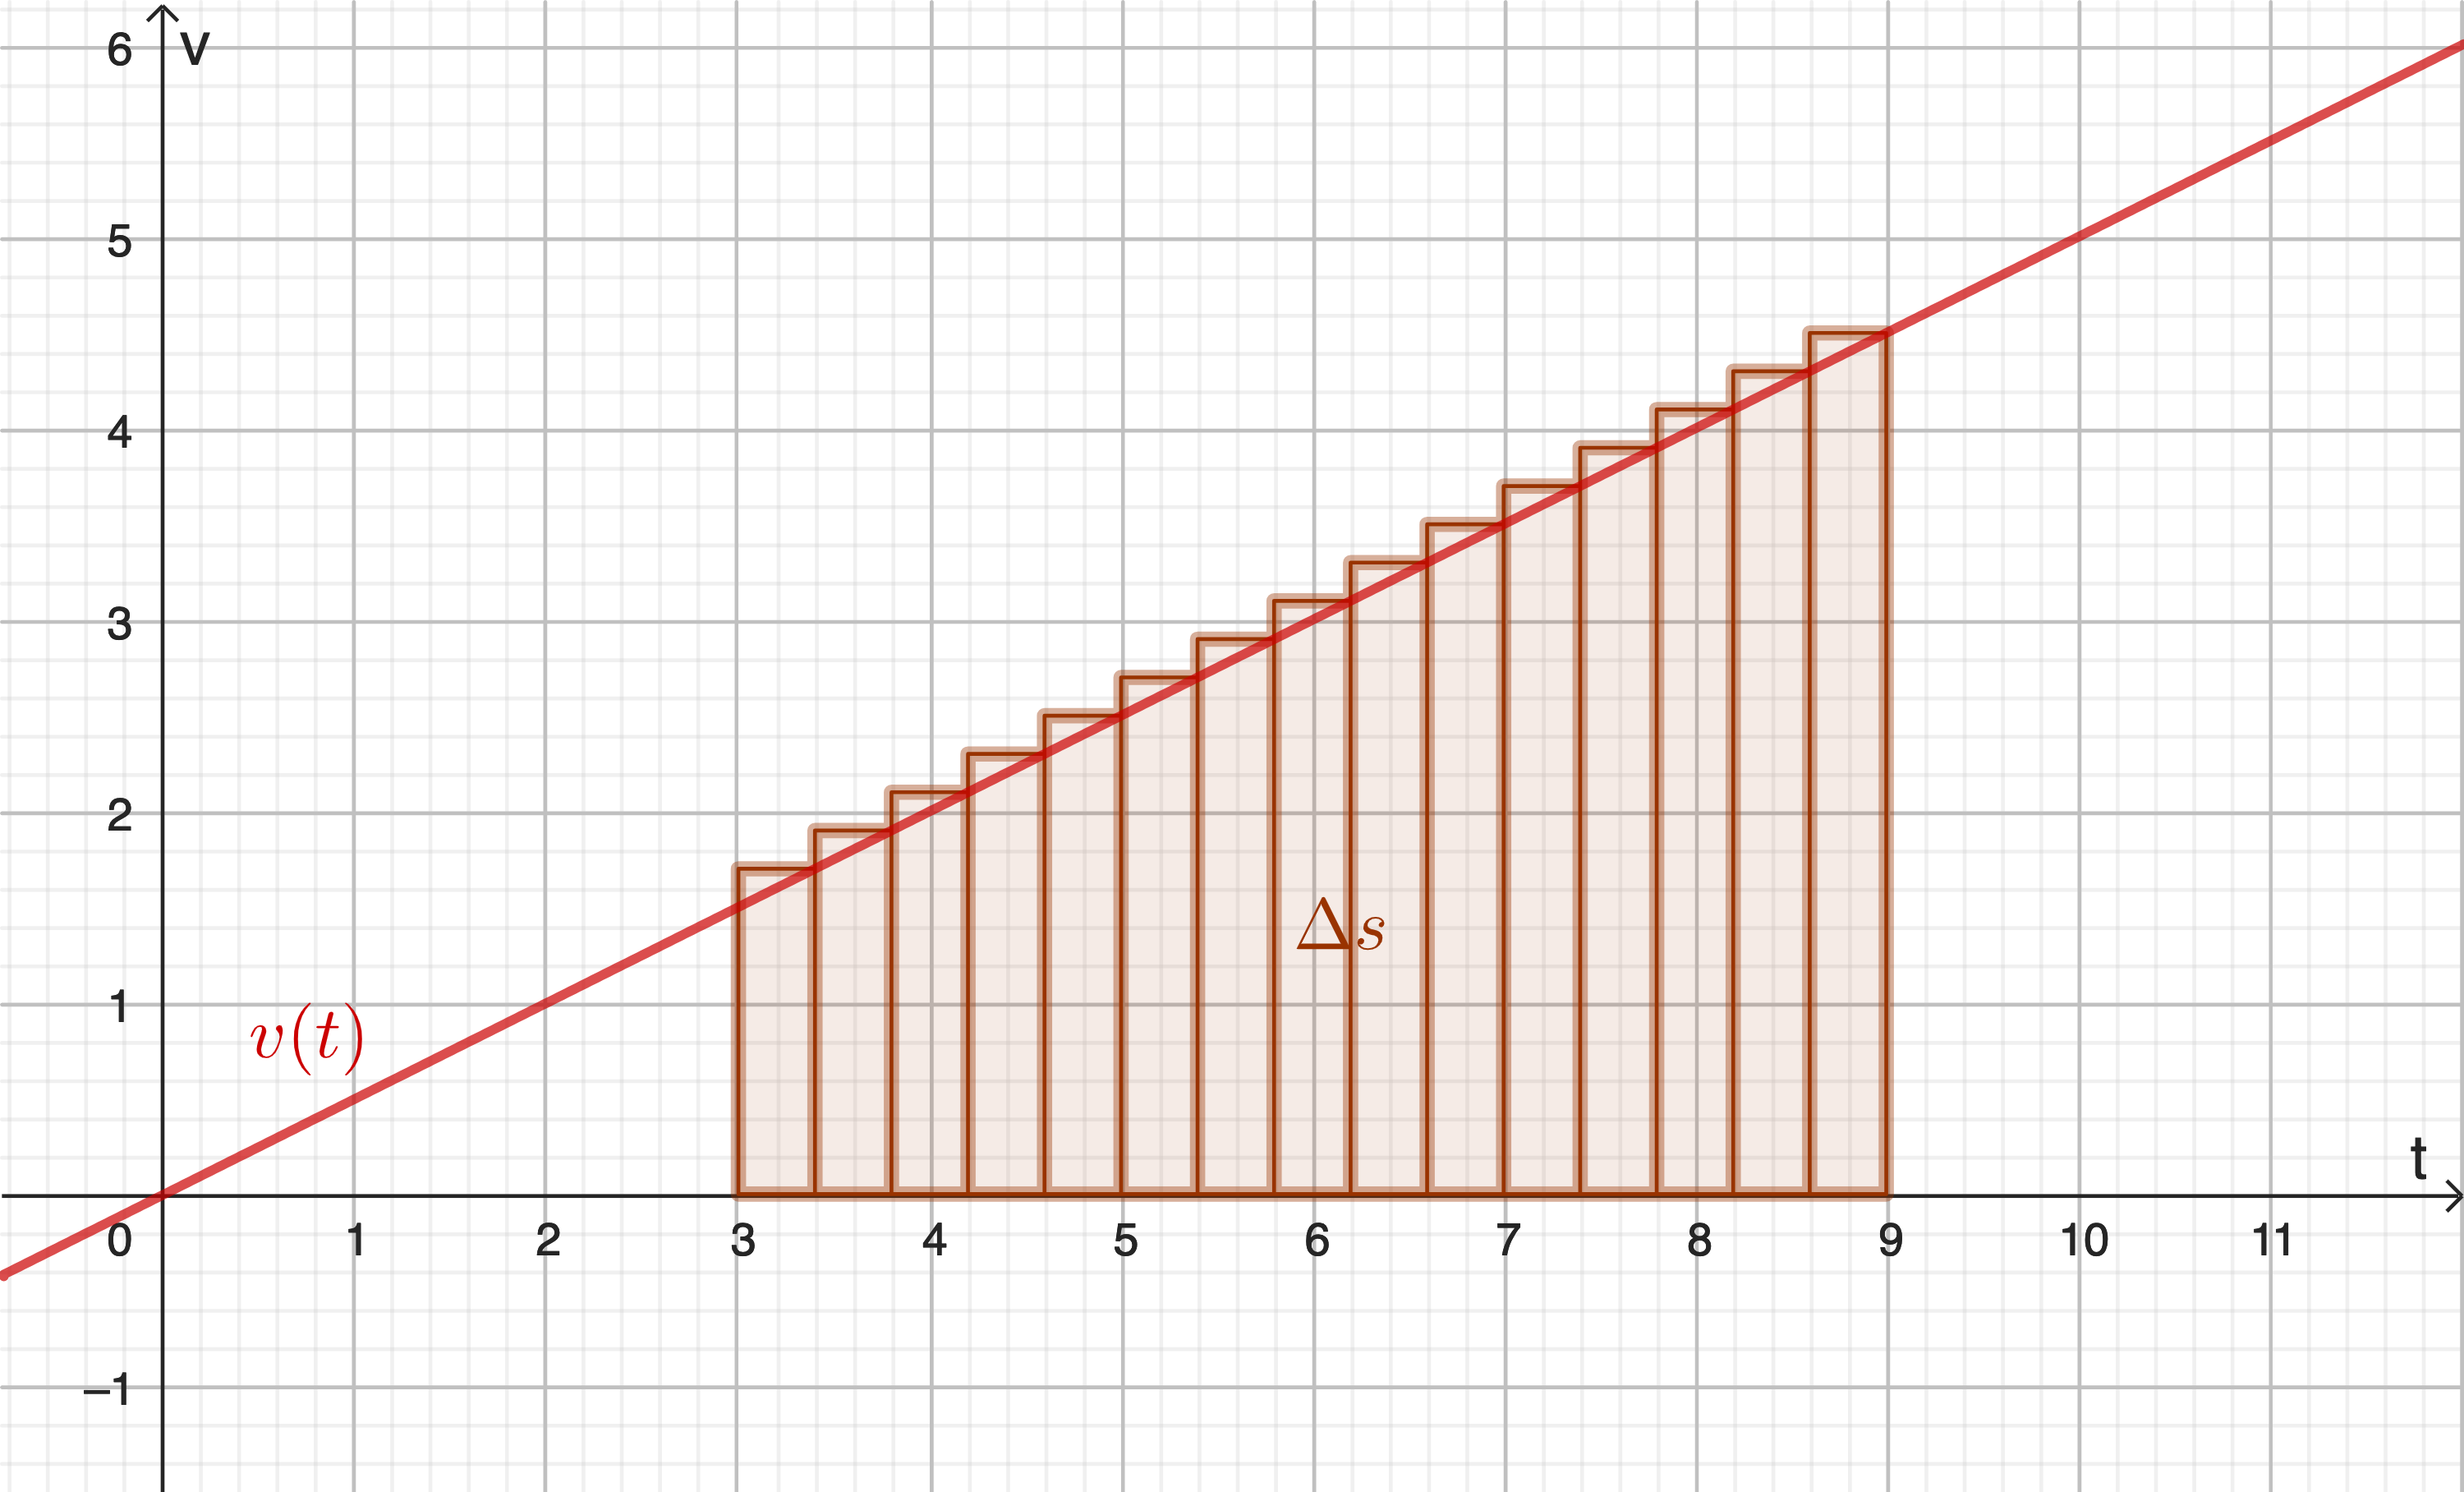
\includegraphics[width = 0.5\textwidth]{media/WegAlsIntegral2.png}
\end{center}
Diese Näherung ist umso besser, je kleiner und zahlreicher die Zeitintervalle werden. Im Grenzfall erhalten wir:
$$\Delta s = \int_{t_1}^{t_2} v(t) \,dt =  \int_{t_1}^{t_2} (a\cdot t) \,dt = \frac{1}{2}at_2^2-\frac{1}{2}at_1^2$$
 
\begin{satz}
    {Zurückgelegter Weg als Integral der Geschwindigkeit}{}
    Allgemein gilt:
    $$\Delta s = \int_{t_1}^{t_2} v(t) \,dt$$
\end{satz}

Die gleiche Überlegung stimmt auch für die mechanische Arbeit:

Die Energie, welche benötigt wird, um einen Körper gegen eine wirkende Kraft zu bewegen, wird in der Physik Arbeit genannt. Wenn die Kraft konstant ist, entspricht die Arbeit $W$ dem Produkt aus Kraft und Weg:
$W=F\cdot \Delta s$
\begin{bsp}
    {Arbeit bei konstanter Kraft}{}
    Welche Arbeit muss geleistet werden, um eine Masse $m$ von der Erdoberfläche auf die (geringe) Höhe $h$ zu bringen?

    Zurückgelegter Weg: \(\Delta s = h\)

    Wirkende Kraft (in der Nähe der Erdoberfläche): \(F = mg\)  mit $g \approx 9.81 m/s^2$

    Die Arbeit ist also
    \[W = mgh\]
    Die Arbeit entspricht gerade der potentiellen Energie einer Masse \(m\) auf der Höhe \(h\).
    Grafisch kann das Produkt aus Kraft und Weg wieder als Flächeninhalt interpretiert werden:
    \begin{center}
        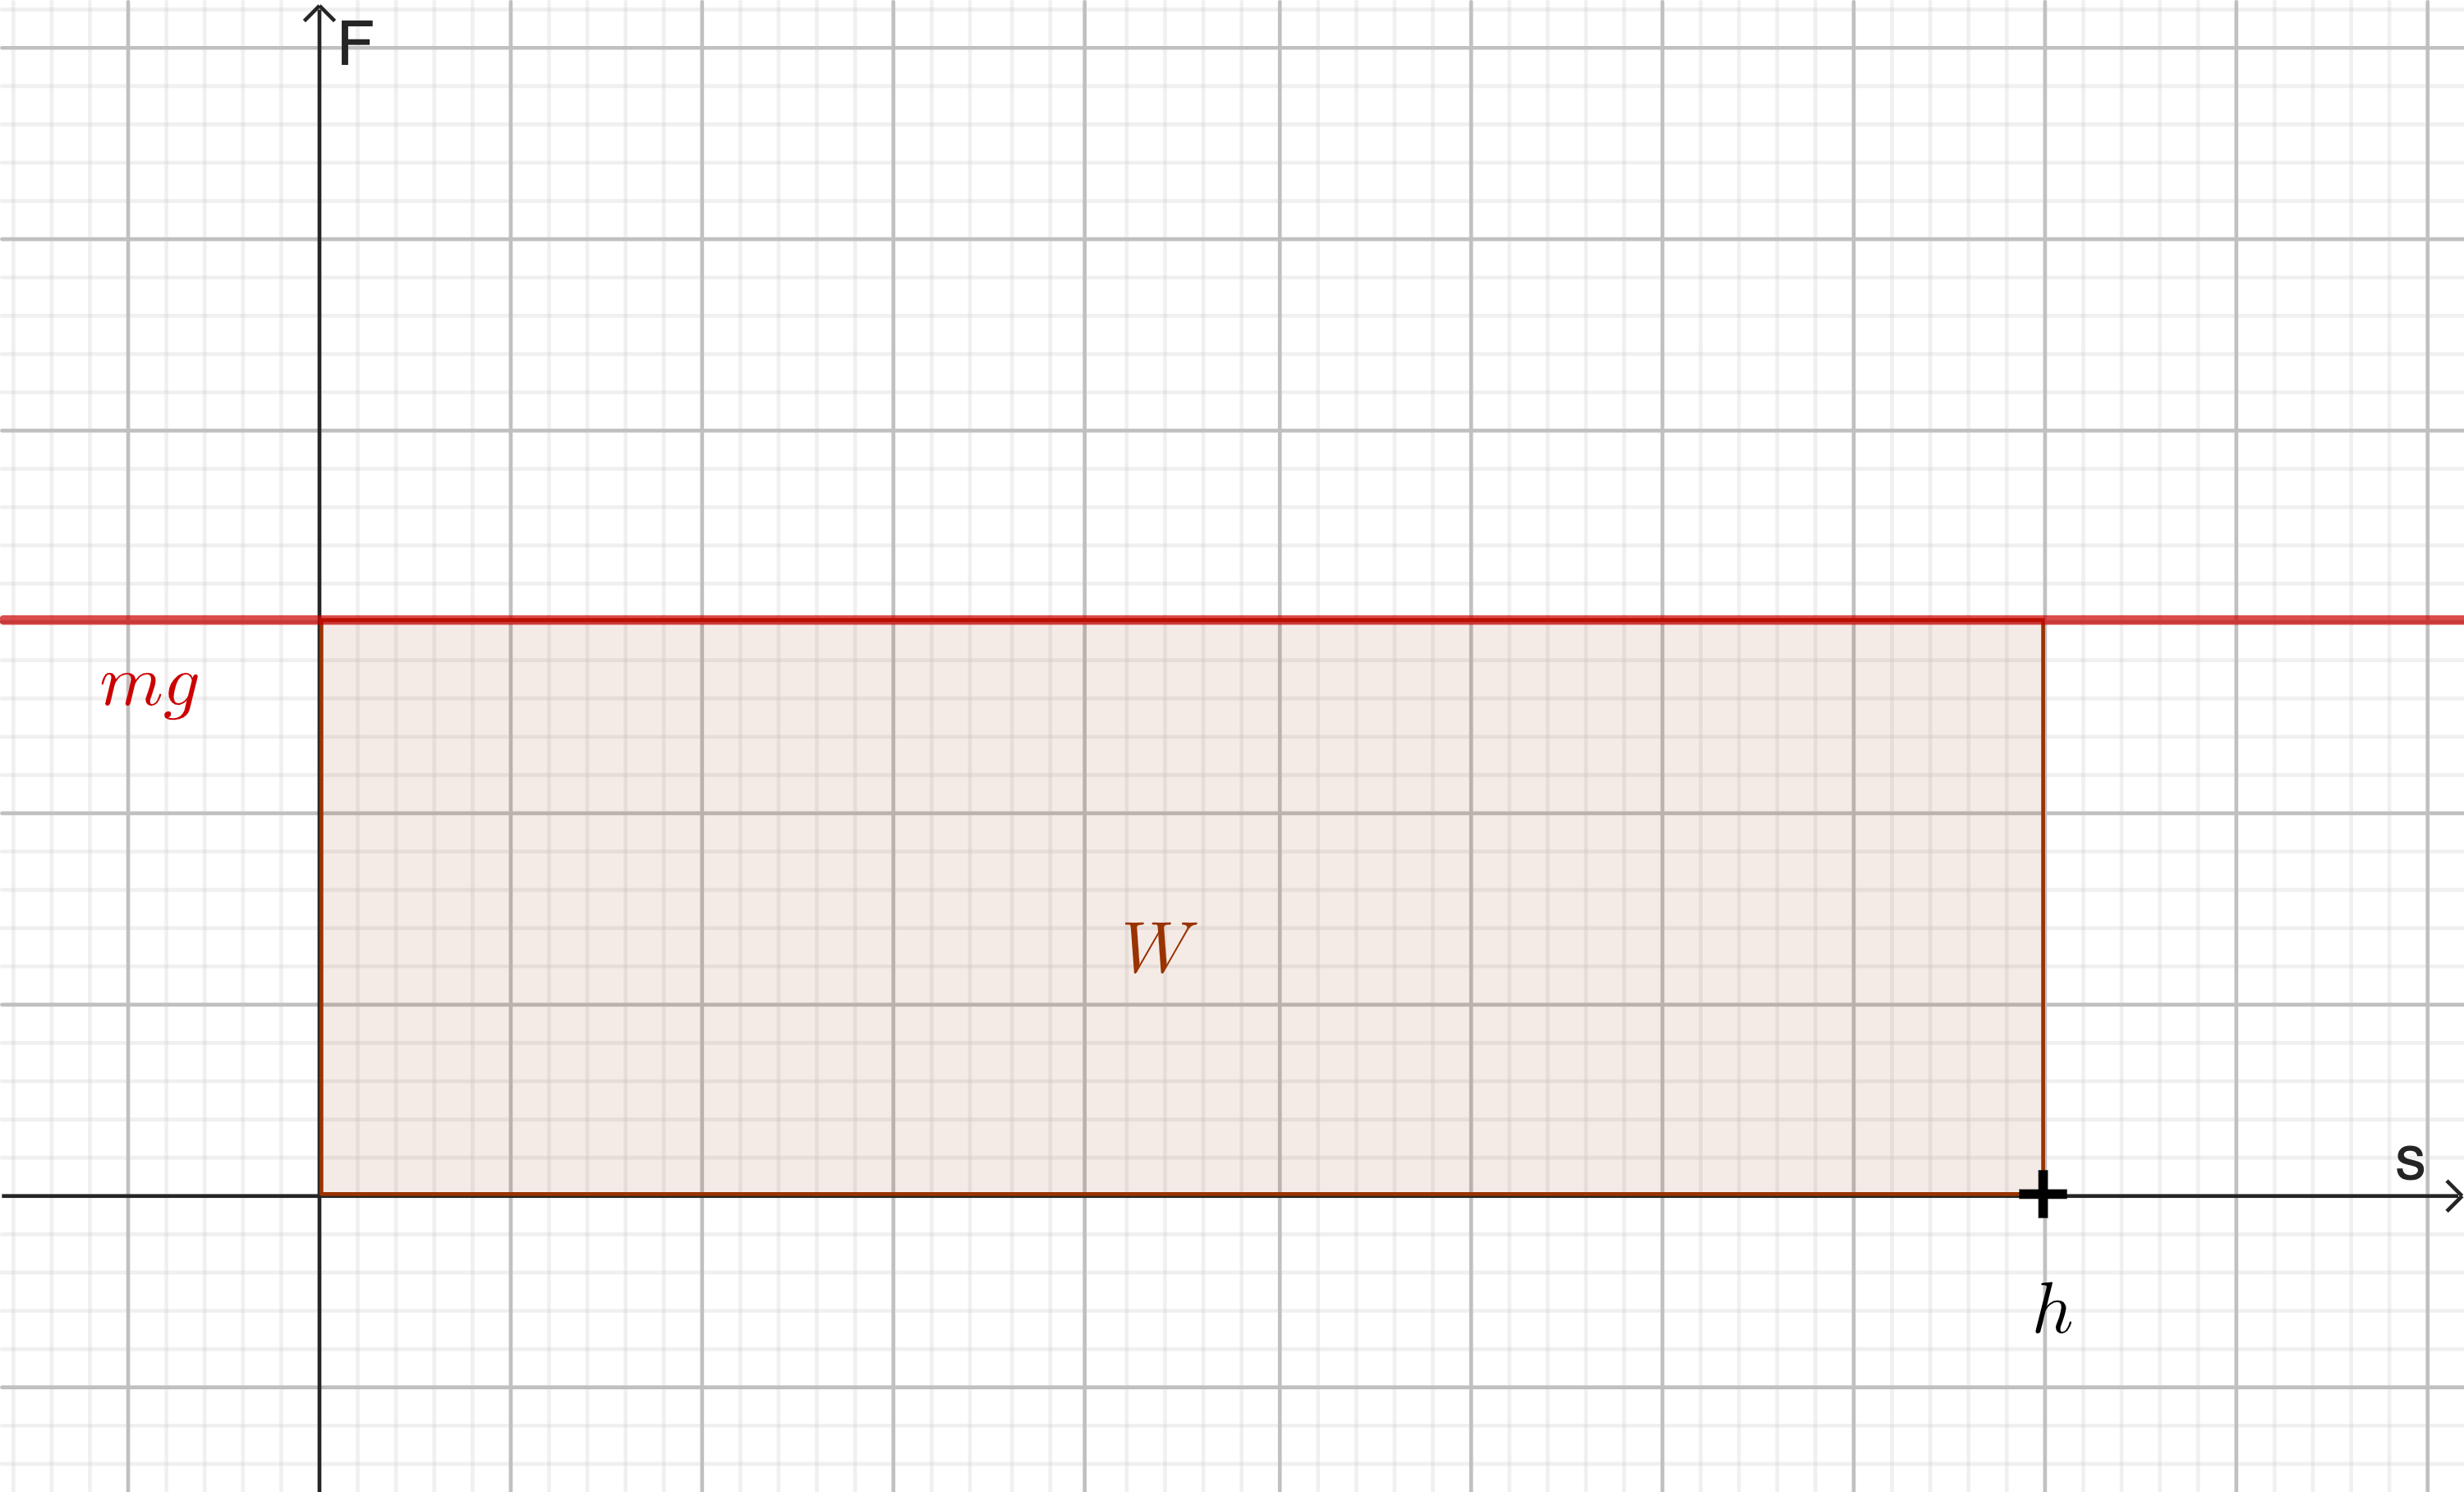
\includegraphics[width = 0.5\textwidth]{media/arbeitAlsIntegral1.png}
    \end{center}

\end{bsp}
\begin{bsp}
    {Arbeit bei linear wachsender Kraft}{}
    Eine Feder mit der Federkonstante \(k\) wird aus der Ruhelage um die Strecke \(a\) gespannt. In diesem Beispiel ist die wirkende Kraft \(F\) proportional zur Auslenkung \(x\) der Feder: \(F = k \cdot x\), wobei $k$ die Federkonstante ist. Um die Arbeit näherungsweise zu berechnen, teilen wir die Strecke \(\Delta s = a\) in viele kleine Intervalle und nehmen an, dass in diesen kleinen Wegintervallen die wirkende Kraft näherungsweise konstant ist.

    \begin{center}
        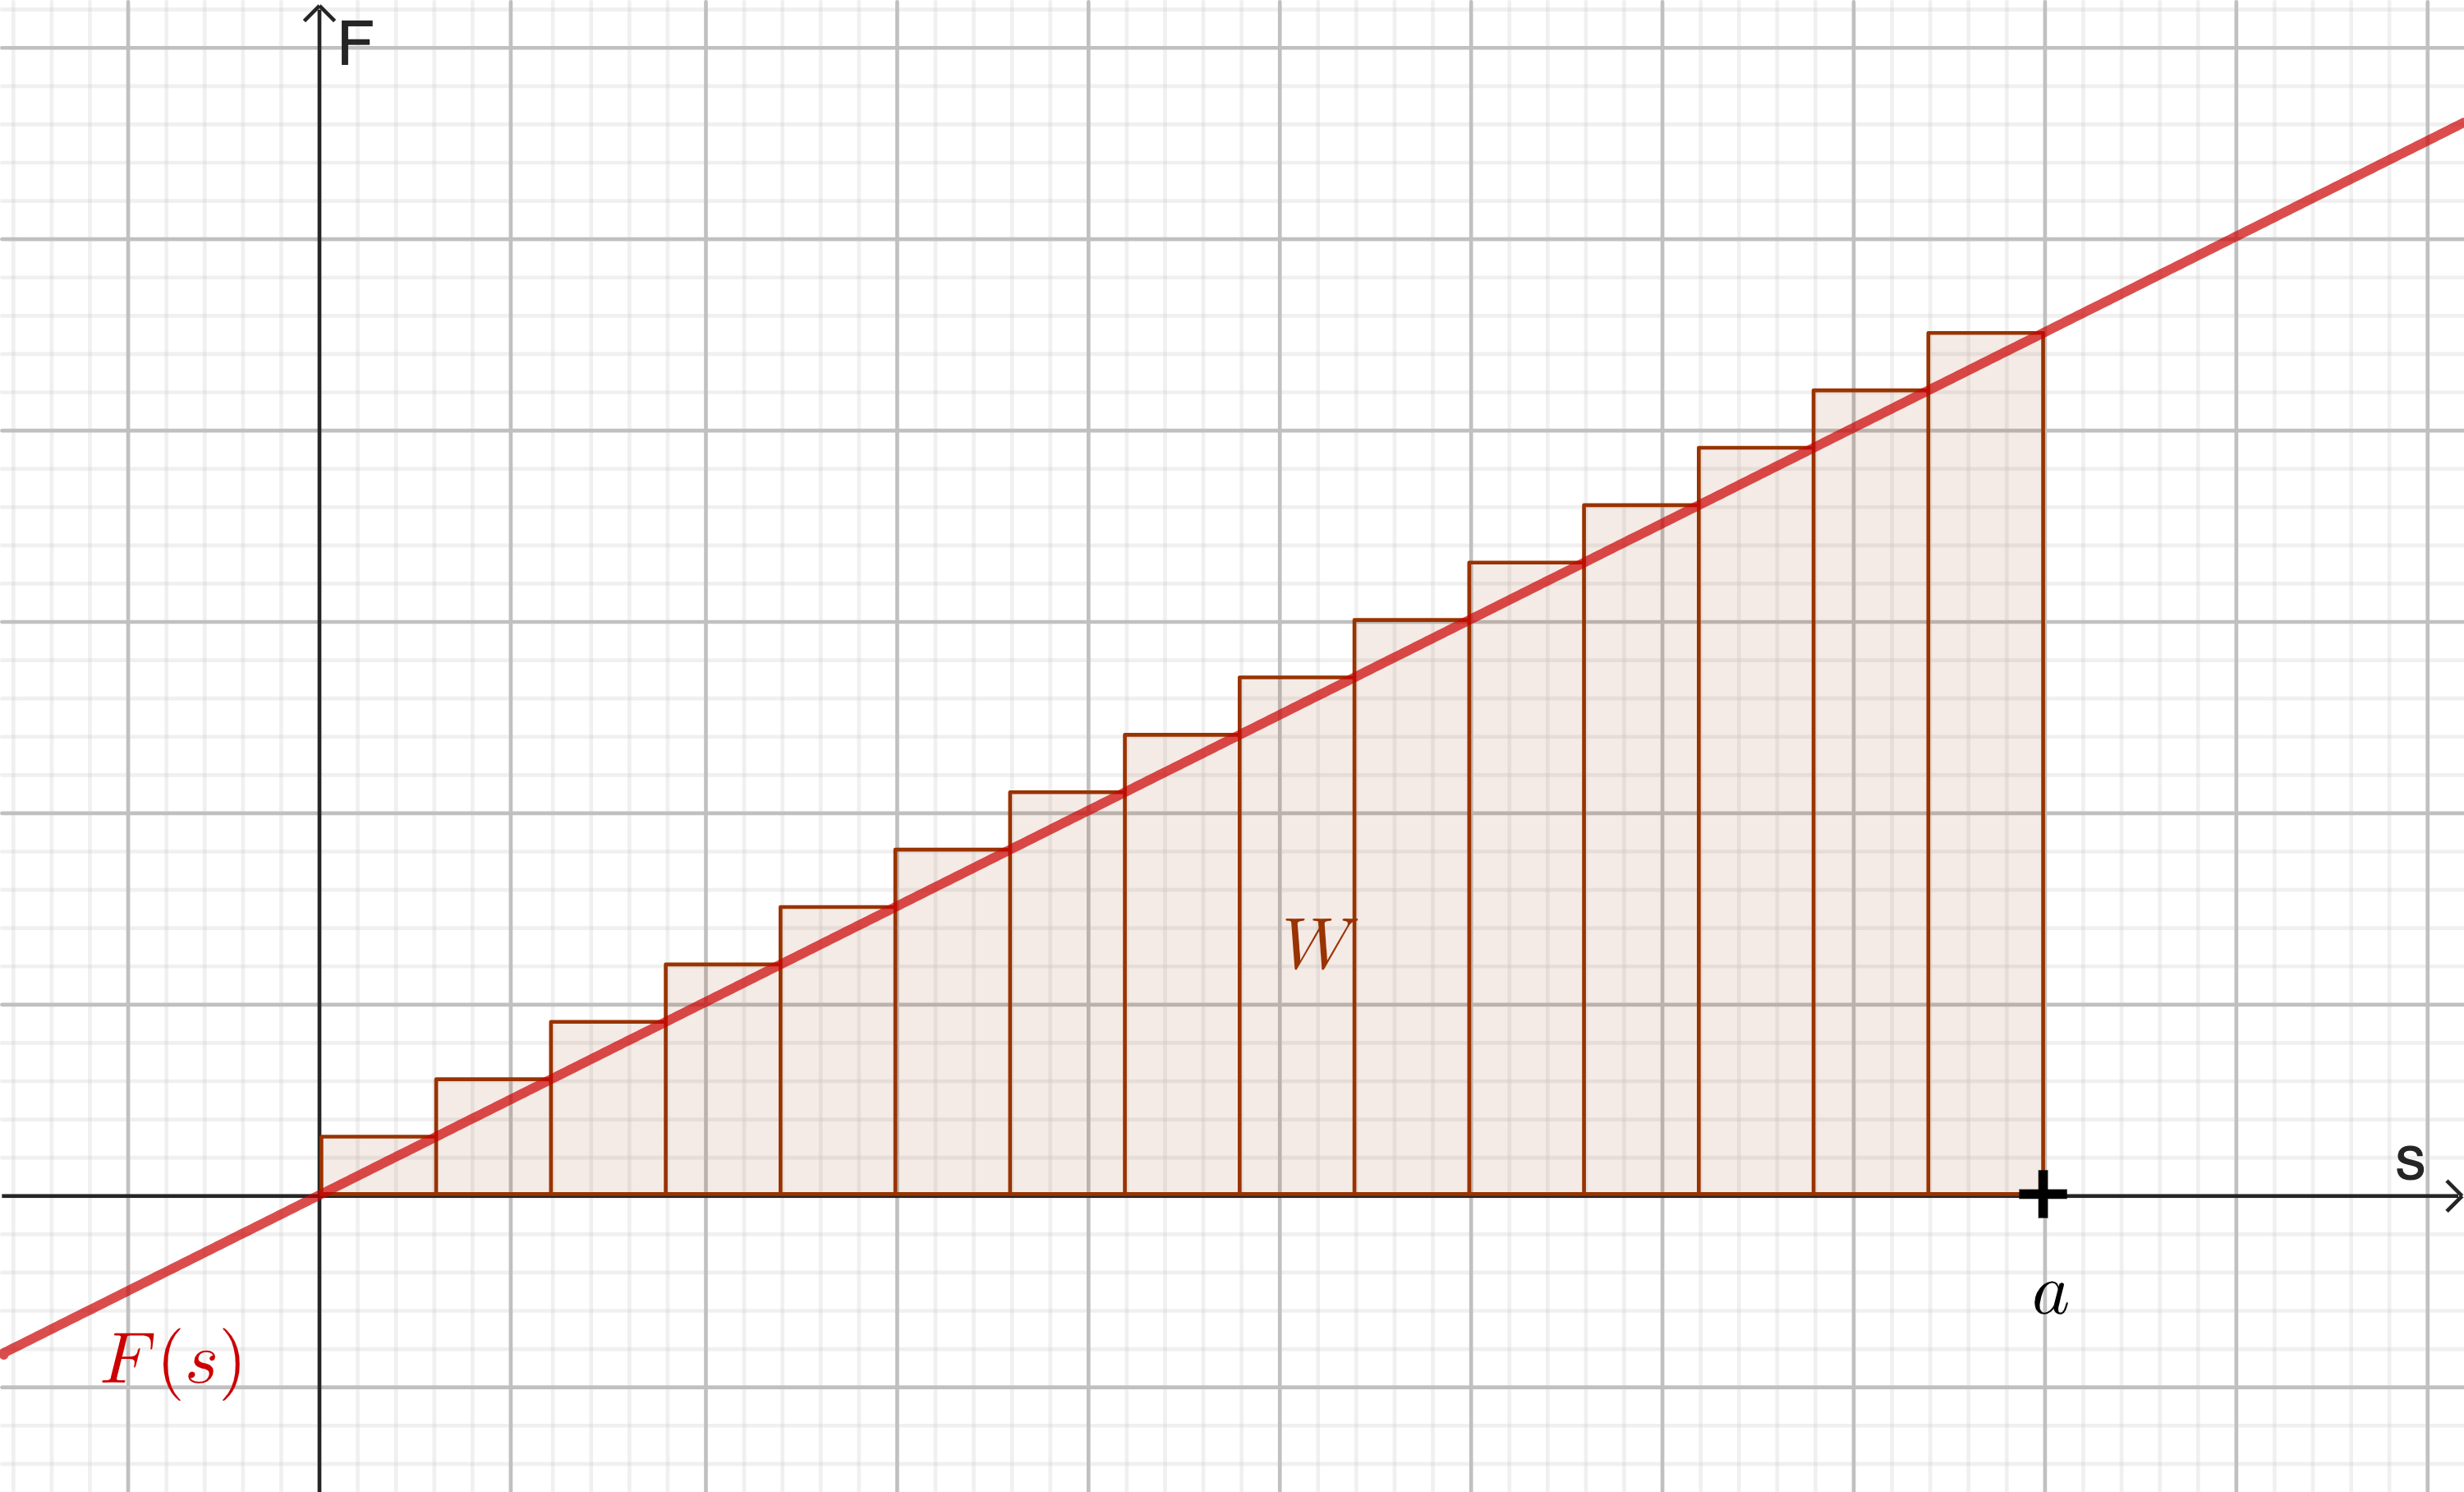
\includegraphics[width = 0.5\textwidth]{media/ArbeitAlsIntegral2.png}
    \end{center}

    Diese Näherung wird umso besser, je kleiner und zahlreicher die Wegintervalle werden. Im Grenzfall erhalten wir:
    \[ W = \int_{0}^{a} F(s) \, ds = \frac{k}{2} a^2 \]

\end{bsp}
\begin{satz}
    {Mechanische Arbeit als Integral}{}
    Allgemein gilt
    $$W = \int_{s_1}^{s_2} F(s) \, ds$$
\end{satz}
